\chapter{\label{chap:experimentation-and-results}Experimentação e Resultados
Obtidos}
Neste capítulo, detalhamos os experimentos que executamos para testar a eficácia
da técnica \textit{NEAT} para navegação em \textit{Spelunky}. Na seção
\ref{section:test-rig}, descrevemos as configurações relevantes de
\textit{hardware} e \textit{software} das máquinas que utilizamos para rodar os
experimentos. Na seção \ref{section:fitness-experiment} apresentamos os
resultados dos testes de funções de aptidão iniciais que escolhemos. Na seção
\ref{section:obstacle-experiment} expomos os resultados após a adição do
neurônio de obstáculo. Na seção \ref{section:experiment-vision} indicamos os
resultados obtidos ao modificarmos o tamanho de área de visão. Nas seções
\ref{section:experiment-extra1}, \ref{section:experiment-extra2} e
\ref{section:experiment-extra3}, exibimos os resultados dos cenários de testes
específicos, descritos previamente na seção \ref{section:scenarios-specific}.

%----------
\section{\label{section:test-rig}Ambiente de Execução}
O capítulo \ref{chap:development} explica que fizemos a execução do jogo em um
ambiente dedicado, utilizando o sistema operacional \textit{Linux}. Para isso,
utilizamos a plataforma \textit{Digital
Ocean}\footnote{https://www.digitalocean.com/}, que facilita a criação de uma
máquina para uso nesse trabalho. Além disso, essa plataforma permite alterar as
configurações -- quantidade de memória, número de processadores e quantidade de
armazenamento -- das máquina a qualquer momento, o que nos permitiu testar
diferentes configurações para o nosso problema.

Conforme explicado na seção \ref{sub:virtual-display}, fazemos o uso do
\textit{XVFB} para permitir a execução do jogo em um \textit{display} virtual. A
utilização de um \textit{display} virtual significa que necessitamos de uma
quantidade razoável de memória na máquina, sendo este um dos recursos mais
importantes para nós. Embora façamos a gravação de algumas informações em disco,
tratam-se apenas de arquivos de texto, que não ocupam uma grande quantidade de
espaço. Tendo isso em consideração, optamos por utilizar \textbf{3} máquinas,
com as configurações exibidas a seguir:

\begin{description}
    \item [Sistema Operacional] Ubuntu 16.04 - 64 \textit{bits}
    \item [Número de Processadores] 4
    \item [Modelo do Processador] Intel(R) Xeon(R) CPU E5-2630L v2 @ 2.40GHz
    \item [Quantidade de Memória] 4GB
    \item [Tipo de Disco] SSD
    \item [Quantidade de Disco] 60GB
\end{description}

Para automatizar o processo de configuração dessas máquinas, fizemos um
\textit{script} de instalação\footnote{https://github.com/famw/provisioning} de
todas as dependências para executar o projeto. Isto faz com que seja fácil
configurar uma nova máquina capaz de executar o treinamento dos agentes.


%----------
\section{\label{section:experiments}Experimentos Realizados}

\subsection{\label{section:fitness-experiment}Escolha da Função de Aptidão}
Conforme vimos na seção \ref{section:modelling-fitness}, A função de aptidão é o
que determina a \textbf{qualidade} da execução de um agente inteligente que
utiliza algoritmos genéticos. Portanto, é de extrema relevância experimentarmos
diferentes funções de aptidão para descobrirmos qual se encaixa melhor no nosso
problema. Assim, fizemos a execução do \textit{bot} no cenário \textbf{fácil}
(Figura \ref{fig:level1}, Capítulo \ref{chap:scenarios}) com três diferentes
funções de aptidão: \textbf{média aritmética}, \textbf{média aritmética
ponderada} e \textbf{média harmônica}, representadas pelas Equações
\ref{eq:fitness-mean}, \ref{eq:fitness-weighted-mean} e
\ref{eq:fitness-harmonic-mean}, respectivamente. Obtivemos os resultados
apresentados na Figura \ref{fig:fitness-experiment}.

\begin{figure}[H]
\centering
	\begin{subfigure}[b]{0.45\textwidth}
        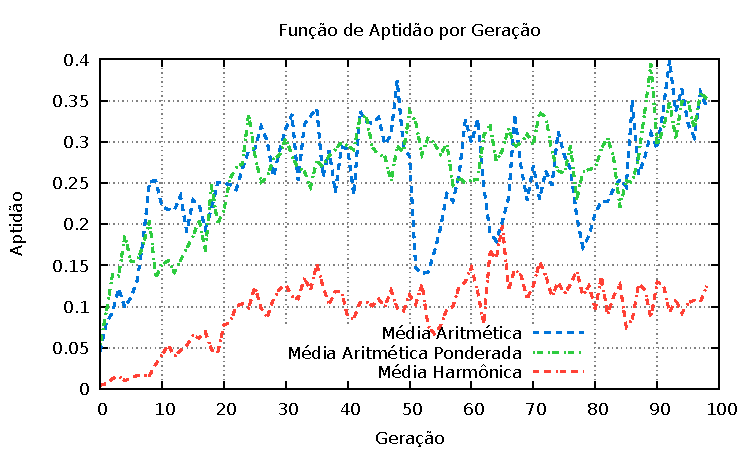
\includegraphics[width=\textwidth]{fig/fitness-value-comparison.pdf}
		\caption{Valor de aptidão médio dos organismos em função do número de
		gerações para as diferentes funções de aptidão escolhidas.}
	\end{subfigure}
	\begin{subfigure}[b]{0.45\textwidth}
        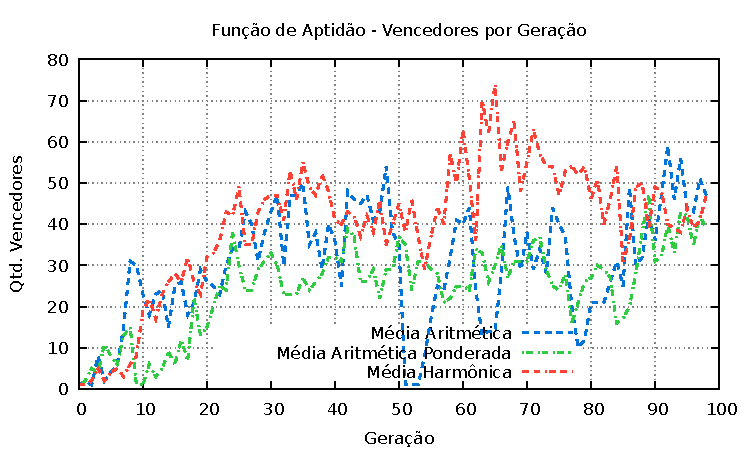
\includegraphics[width=\textwidth]{fig/fitness-winners-comparison.pdf}
        \caption{Número de organismos vencedores por geração para as diferentes
        funções de aptidão escolhidas.}
		\label{fig:fitness-experiment-winners}
	\end{subfigure}

    \caption{Resultado da execução do cenário fácil com diferentes funções de
    aptidão.}
	\label{fig:fitness-experiment}
\end{figure}

Através da análise dos resultados, é possível perceber que a média
artimética e a média aritmética ponderada possuem um comportamento muito
similar, mas os resultados de número de vencedores e aptidão média da média
aritmética ponderada foram mais estáveis.

A Figura \ref{fig:fitness-experiment-winners} nos indica que a média harmônica
foi capaz de gerar um número de vencedores muito similar ao das outras funções,
mesmo que seus valores de média de aptidão sejam bem inferiores aos das demais.
Este comportamento pode ser explicado da seguinte maneira: a média harmônica
possui uma tendência natural de calcular um valor de média inferior aos valores
gerados pelas outras médias. Essa escala reduzida de valores, portanto, não é um
problema, pos todos os organismos são classificados utilizando a mesma função.

Considerando os resultados obtidos, escolhemos ficar com a \textbf{média
aritmética ponderada}, por ser uma função que nos oferece um controle maior
sobre os valores que a compôem. Embora a média harmônica tenha apresentado um
comportamento bastante estável para este cenário de teste, não a escolhemos por
dois motivos. Primeiro, a função possui uma tendência de produzir valores muito
baixos.  Como os cenários de teste adiante são maiores, isto pode vir a
dificultar os treinamentos. Segundo, como nossos valores de aptidão estão sempre
normalizados entre o intervalo $[0,1]$, os valores extremamente baixos que a
média harmônica gera podem acarretar em uma perda de precisão numérica.

\subsection{\label{section:obstacle-experiment}Adição de \textit{Input} de
Obstáculo}

Com a função de aptidão escolhida e o nível fácil superado, o próximo passo foi
executar o treinamento dos agentes no nível \textbf{médio}. Os resultados desta
execução são apresentados na Figura \ref{fig:medium-wam-experiment}.

\begin{figure}[H]
\centering
	\begin{subfigure}[b]{0.45\textwidth}
        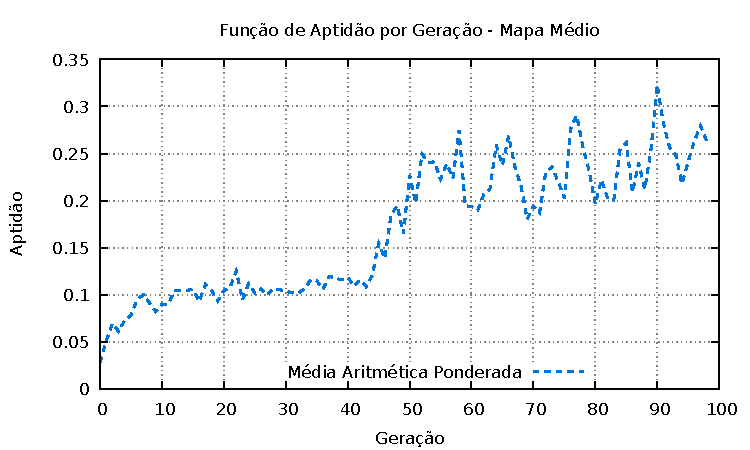
\includegraphics[width=\textwidth]{fig/medium-wam-fitness-experiment.pdf}
        \caption{Valor de aptidão em função do número de gerações para a média
        aritmética ponderada no mapa médio.}
	\end{subfigure}
	\begin{subfigure}[b]{0.45\textwidth}
        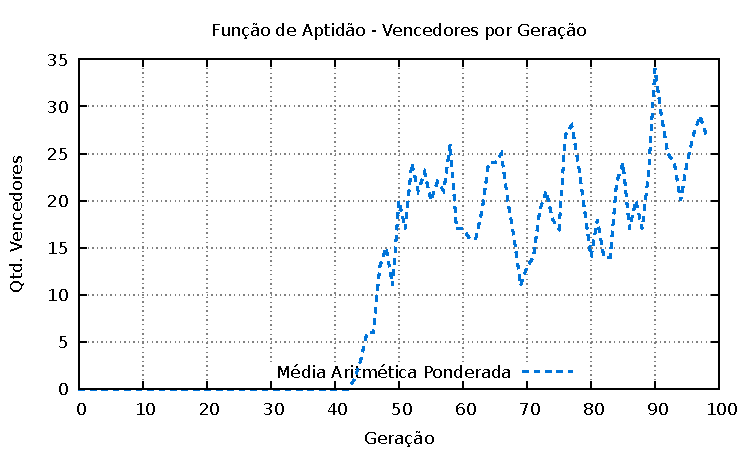
\includegraphics[width=\textwidth]{fig/medium-wam-winners-experiment.pdf}
        \caption{Número de organismos vencedores por geração para a média
        aritmética ponderada no mapa médio.}
	\end{subfigure}

    \caption{Resultado da execução do cenário médio com a média aritmética
    ponderada.}
	\label{fig:medium-wam-experiment}
\end{figure}

Inicialmente, não realizamos nenhuma modificação nas configurações, executando
exatamente o mesmo programa do nível anterior. O algoritmo foi capaz de
encontrar uma solução, contudo percebemos que os organismos demoravam muito
tempo para chegar até o final do nível.  Acompanhando a execução, vimos que em
muitas gerações o \textit{bot} ia, no máximo, até o local indicado pela Figura
\ref{fig:experiment-medium-stuck}.

\begin{figure}[htb!]
\centering
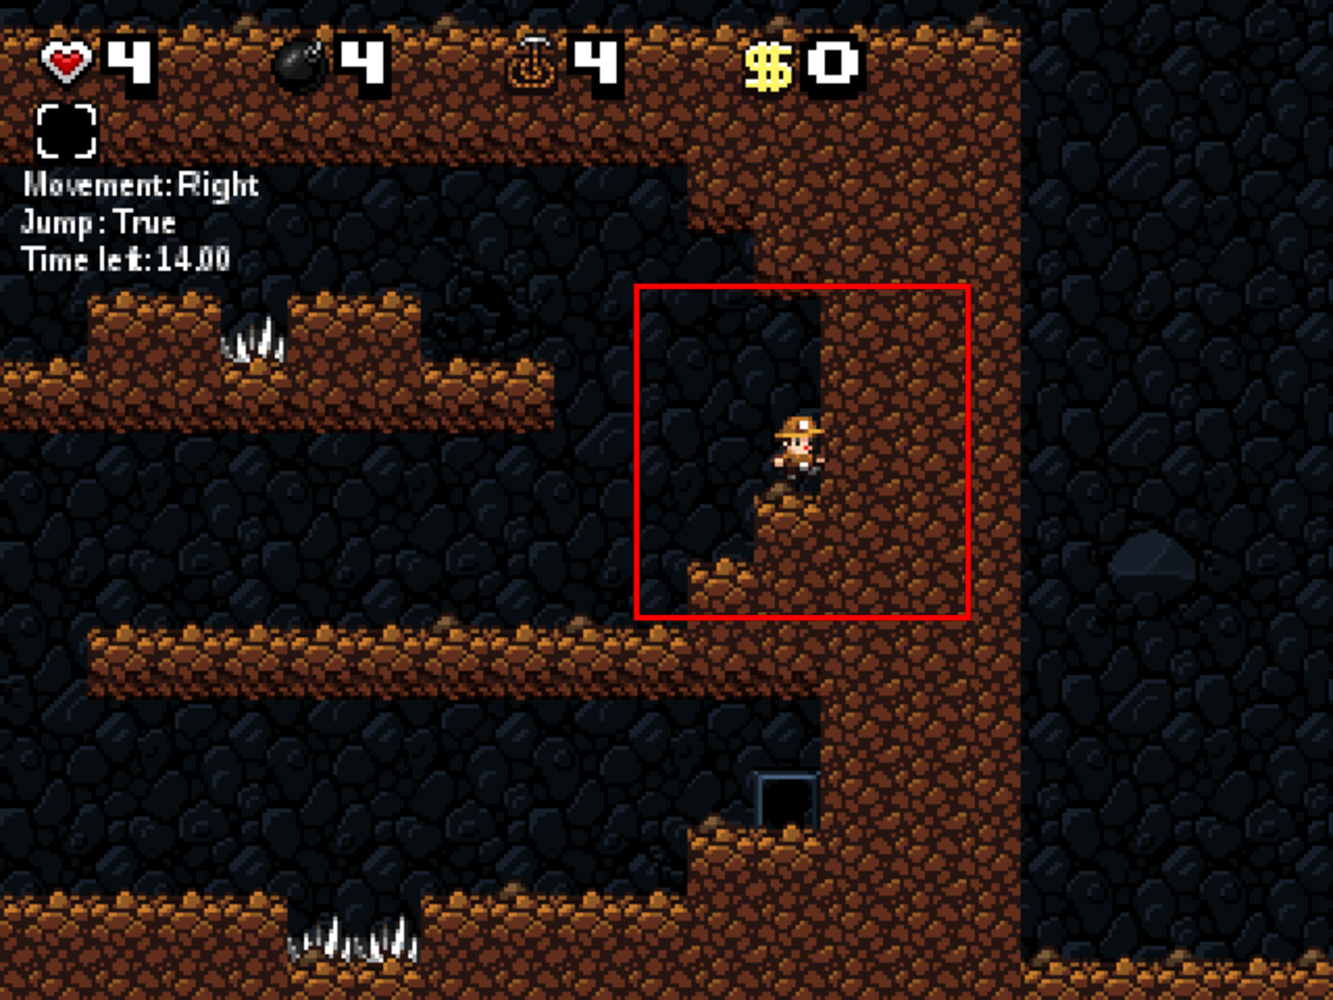
\includegraphics[width=.5\textwidth]{fig/experiment-medium-stuck.pdf}
\caption{Experimento mostrando o local onde o \textit{bot} fica parado ao
    executar no mapa médio com a média aritmética ponderada como função de
    aptidão.}
\label{fig:experiment-medium-stuck}
\end{figure}

Analisamos esse comportamento e percebemos que os agentes estavam em um local
que, até naquele momento, era considerado como \textit{ótimo}.  Identificamos
uma possível causa deste fenômeno: a parte do cálculo de distância de nossa
função de aptidão produz valores mais altos quanto maior for o deslocamento
horizontal e vertical do agente. Desta forma, os organismos identificaram que,
caso se deslocassem para a esquerda, o valor de aptidão seria pior do que se
permanecessem parados na região indicada.

O valor de aptidão só viria a ser maior do que este ótimo local caso os agentes
se deslocassem ao máximo para a esquerda, caindo para o primeiro ``andar'' do
mapa, pois assim o deslocamento no eixo $y$ compensaria o esforço. Foi
necessário um número grande de iterações do algoritmo até que, finalmente, uma
combinação de mutações resultasse em um organismo vencedor.

Mesmo que o algoritmo tenha sido capaz de criar um agente vencedor, foi preciso
muito tempo de execução para tal (mais de 40 iterações). Portanto, visando fazer
com que os organismos aprendessem mais rapidamente, adicionamento a entrada de
\textit{obstáculo} na rede, cuja explicação se encontra na seção
\ref{section:obstacle-input}. A Figura
\ref{fig:medium-wam-obs-fitness-experiment} ilustra os resultados desta
modificação e apresenta uma comparação com a execução sem o neurônio de
obstáculo.

\begin{figure}[H]
\centering
	\begin{subfigure}[b]{0.45\textwidth}
        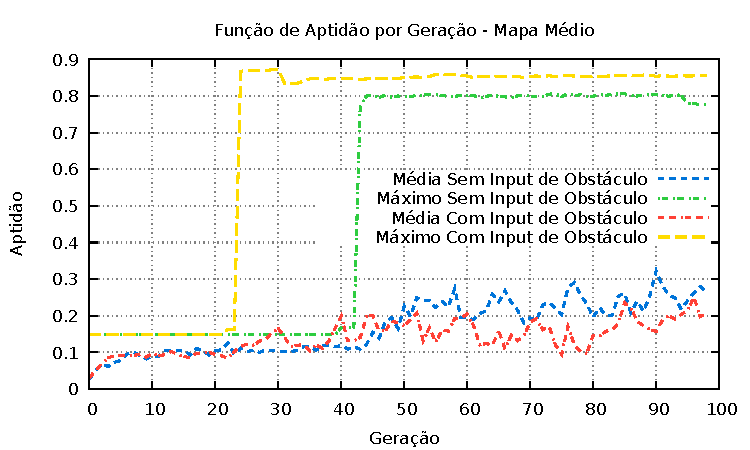
\includegraphics[width=\textwidth]{fig/medium-wam-obs-fitness-experiment.pdf}
        \caption{Valor de aptidão em função do número de gerações para a média
        aritmética ponderada, com o \textit{input} de obstáculo, no mapa
        médio.}
	\end{subfigure}
	\begin{subfigure}[b]{0.45\textwidth}
        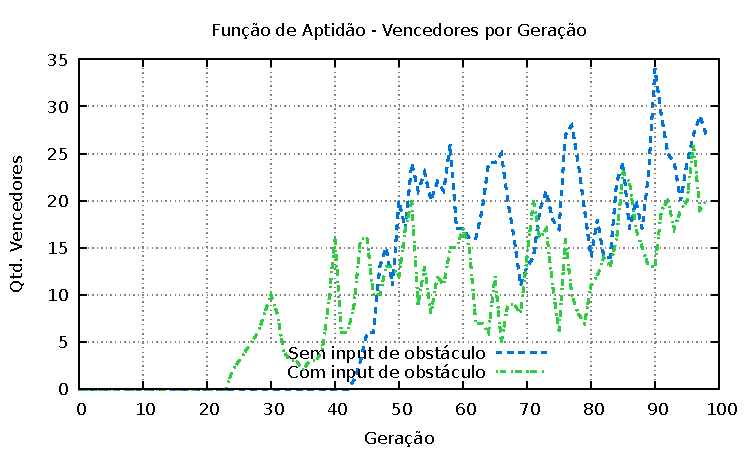
\includegraphics[width=\textwidth]{fig/medium-wam-obs-winners-experiment.pdf}
        \caption{Número de organismos vencedores por geração para a média
        aritmética ponderada, com o \textit{input} de obstáculo, no mapa
        médio.}
	\end{subfigure}

    \caption{Comparação entre os resultados das execuções do cenário médio (com
		média aritmética ponderada) com e sem o neurônio de obstáculo.}
	\label{fig:medium-wam-obs-fitness-experiment}
\end{figure}

Concluímos, então, que a adição dessa nova entrada na rede acelera a capacidade
do algoritmo de encontrar uma solução e fornece um mecanismo capaz de auxiliar
na geração de organismos com aptidão superior. Isto fica evidenciado pelo
surgimento de organismos vencedores próximo da geração de número 20, cortando
pela metade o número de gerações necessárias para encontrar um vencedor, e no
aumento de valor máximo de aptidão dos organismos durante todo o treinamento. 

\subsection{\label{section:experiment-vision}Tamanho da Janela de Visão}

Até então, utilizamos uma configuração de área de visão 5 por 5. Contudo, é
possível que o tamanho da visão do agente influencie positivamente em sua
capacidade de encontrar uma solução mais rápida e eficiente. Acreditamos que
diminuir o tamanho de visão para um tamanho menor que 5 por 5 não traria nenhuma
contribuição significativa, pois o agente se tornaria ``míope'' demais (não
seria capaz nem de enxergar o chão ao pular). Assim, com o objetivo de verificar
se um tamanho de área de visão maior influencia no aprendizado do agente,
executamos novamente o mapa \textbf{médio} utilizando a \textbf{média aritmética
ponderada} e um tamanho de área de visão de 7 por 7.

Observamos que, com as novas configurações, não foi possível gerar nenhum agente
capaz de chegar até o final do nível. Analisando a execução, vimos que muitas
vezes os organismos permaneciam parados em uma determinada posição, ilustrada
pela Figura \ref{fig:experiment-medium-stuck}. É possível perceber que os
agentes conseguiam exergar a porta de saída desta posição. Concluímos, portanto,
que ele não foi capaz de aprender, dentro dos limites de iterações estabelecidos
anteriormente, porque estava visualizando a porta de saída muito precocemente, o
que o influenciava a tomar a decisão de executar a ação de deslocamento para a
direita, essencialmente o ``travando'' em um mesmo local.

\begin{figure}[htb!]
\centering
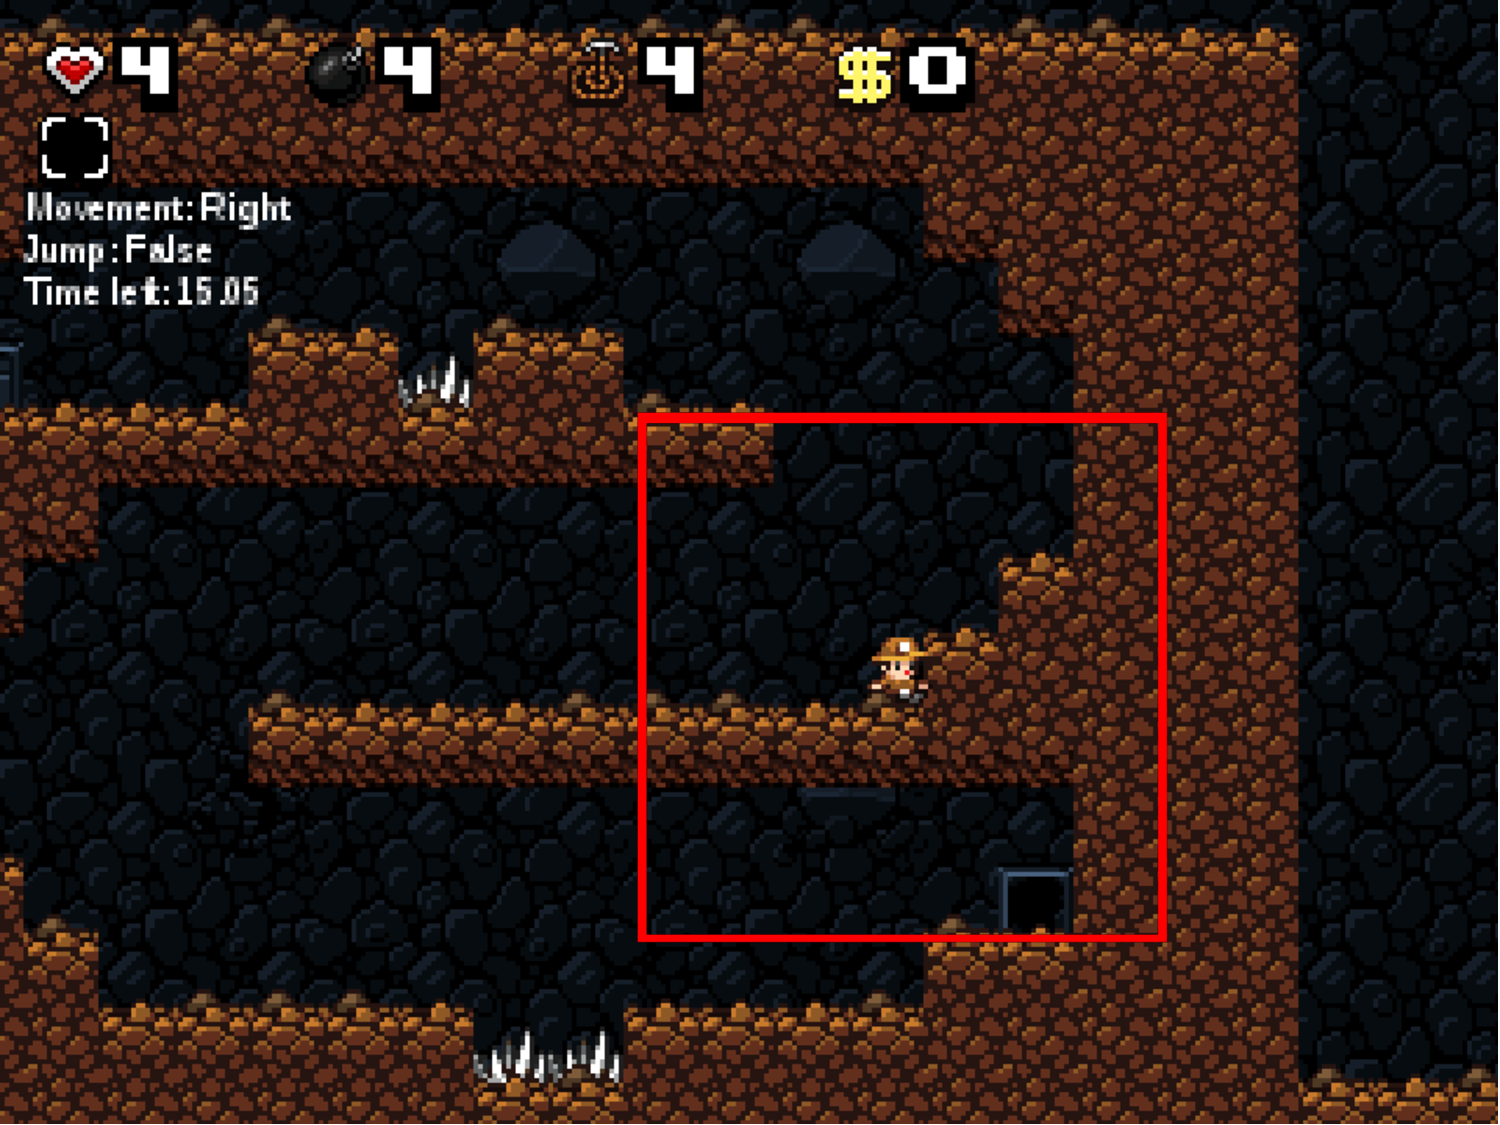
\includegraphics[width=.5\textwidth]{fig/medium-7x7-stuck.pdf}
\caption{Local onde os agentes do experimento de visão permaneciam parados.}
\label{fig:experiment-medium-stuck}
\end{figure}

\subsection{\label{section:experiment-extra1}Execução no Cenário \textit{extra
1}}

O objetivo do cenário \textbf{extra 1} era detectar se os agentes seriam capazes
de evoluir ao ponto de aprenderem a utilizar uma escada, funcionalidade que não
foi explorada até então. Para subir a escada, o jogador deve pressionar o botão
de olhar para cima quando encontrar uma escada, subindo-a enquanto esse botão
estiver pressionado. Para isso, adicionamos a ação de \textbf{olhar para cima}
como saída na rede neural. A Figura \ref{fig:extra1-results} apresenta os
resultados da execução deste cenário.

\begin{figure}[H]
\centering
	\begin{subfigure}[b]{0.45\textwidth}
        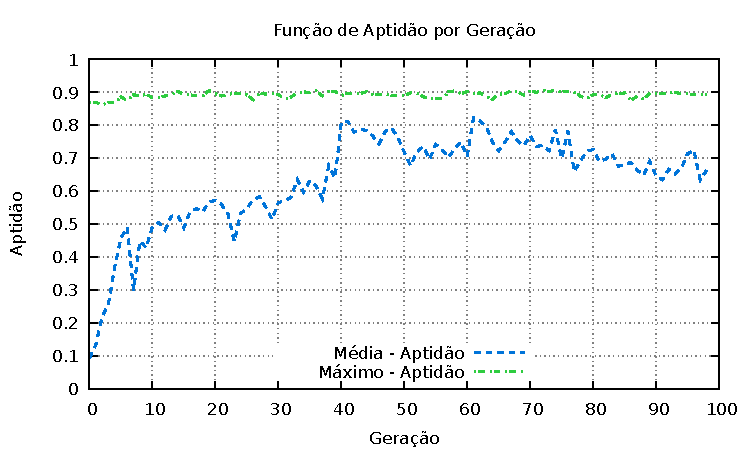
\includegraphics[width=\textwidth]{fig/extra1-fitness.pdf}
        \caption{Aptidão em função do número de gerações para o cenário
        \textit{extra 1}.}
	\end{subfigure}
	\begin{subfigure}[b]{0.45\textwidth}
        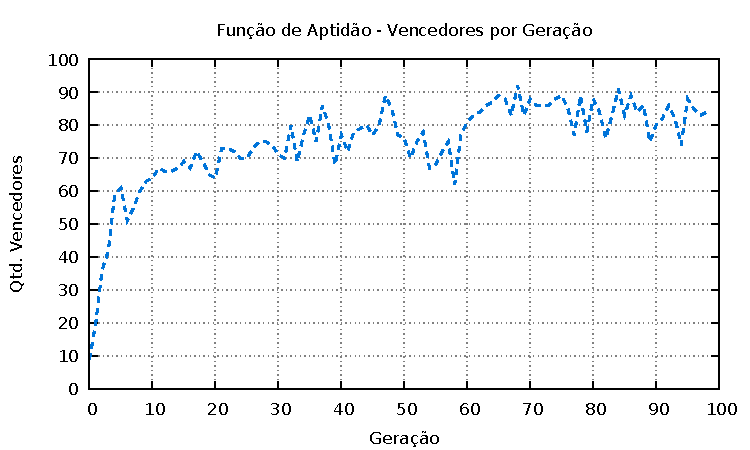
\includegraphics[width=\textwidth]{fig/extra1-winners.pdf}
        \caption{Número de organismos vencedores por geração para o cenário
        \textit{extra 1}.}
	\end{subfigure}

    \caption{Resultado da execução do cenário \textit{extra 1}.}
	\label{fig:extra1-results}
\end{figure}

Analisando os resultados, percebemos que o algoritmo foi capaz de encontrar
agentes vencedores muito rapidamente. Concluímos, portanto, que o resultado
deste experimento é satisfatório, pois isto sinaliza que é possível adicionar
novas capacidades ao agente incrementalmente. Cabe ressaltar, contudo, que caso
desejássemos permitir que os agentes descescem as escadas, seria necessário
adicionar uma outra saída na rede, a de olhar para baixo.

\subsection{\label{section:experiment-extra2}Execução no Cenário \textit{extra
2}}

O cenário \textbf{extra 2} conta com duas paredes que só podem ser puladas caso
o jogador compreenda que deve escalá-las. Assim, este cenário explora a
habilidade do agente de pressionar os botões de \textbf{movimentação} (mesma
direção da parede) e de \textbf{pular} ao mesmo tempo. O resultado da execução
desse nível é apresentado na Figura \ref{fig:extra2-results}.

\begin{figure}[H]
\centering
	\begin{subfigure}[b]{0.45\textwidth}
        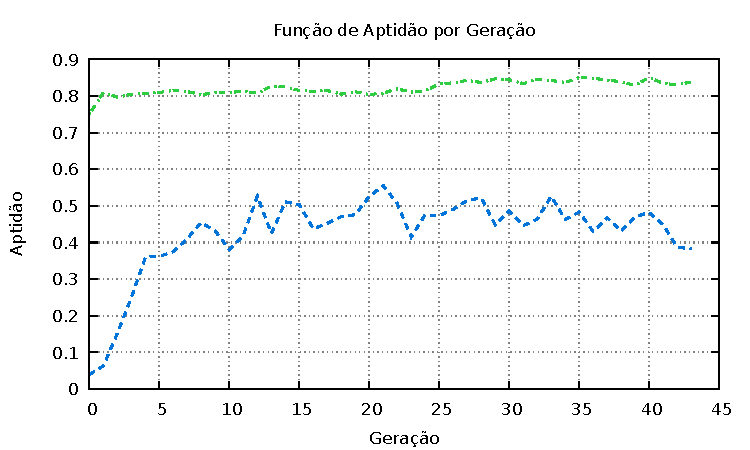
\includegraphics[width=\textwidth]{fig/extra2-fitness.pdf}
        \caption{Aptidão em função do número de gerações para o cenário
        \textit{extra 2}.}
	\end{subfigure}
	\begin{subfigure}[b]{0.45\textwidth}
        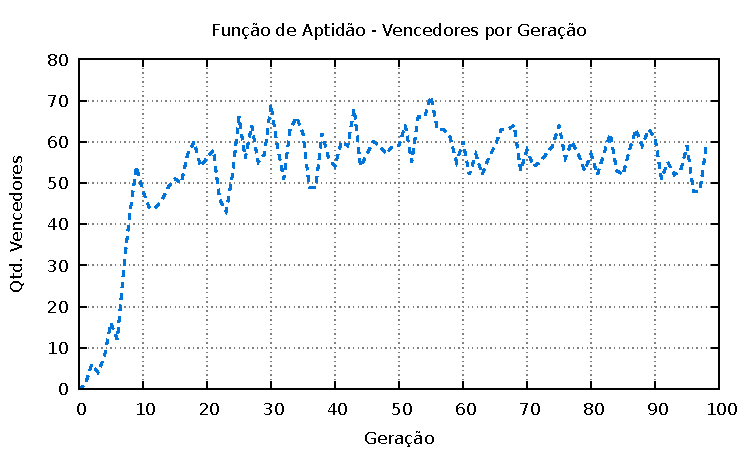
\includegraphics[width=\textwidth]{fig/extra2-winners.pdf}
        \caption{Número de organismos vencedores por geração para o cenário
        \textit{extra 2}.}
	\end{subfigure}

    \caption{Resultado da execução do cenário \textit{extra 2}.}
	\label{fig:extra2-results}
\end{figure}

O resultado da execução é bastante satisfatório. Novamente, os agentes foram
capazes de vencer o nível logo nas primeiras iterações do algoritmo. Além disso,
podemos ver que, após 30 gerações, mais da metade dos organismos foram
vencedores. Por fim, concluímos que nossos agentes são capazes de compreender
que devem combinar ações para atingir alguns objetivos, o que é interessante
para a execução em níveis mais complexos.  

\subsection{\label{section:experiment-extra3}Execução no Cenário \textit{extra
3}}

Em \textit{Spelunky} o jogador pode utilizar a ação de correr para atingir seus
objetivos mais rapidamente. Portanto, o cenário \textbf{extra 3} explora a ação
de correr para gerar o impulso necessário para poder saltar sobre uma região com
espinhos. Para isso, adicionamos a ação de \textbf{correr} na rede neural.  A
Figura \ref{fig:extra3-results} apresenta os resultados da execução deste
cenário.

\begin{figure}[H]
\centering
	\begin{subfigure}[b]{0.45\textwidth}
        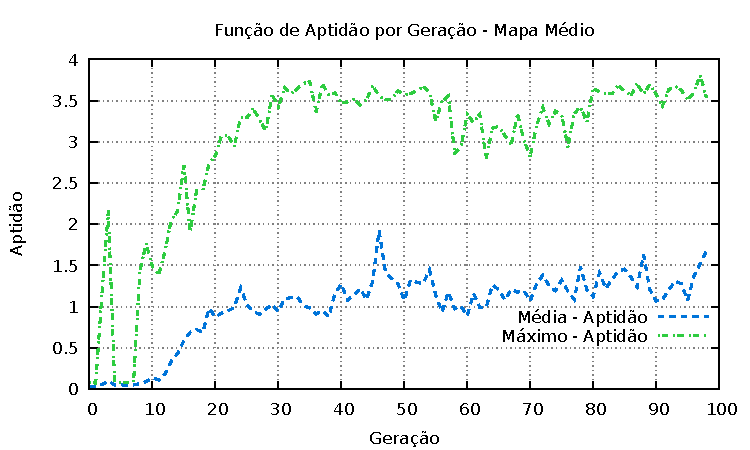
\includegraphics[width=\textwidth]{fig/extra3-fitness.pdf}
        \caption{Aptidão em função do número de gerações para o cenário
        \textit{extra 3}.}
	\end{subfigure}
	\begin{subfigure}[b]{0.45\textwidth}
        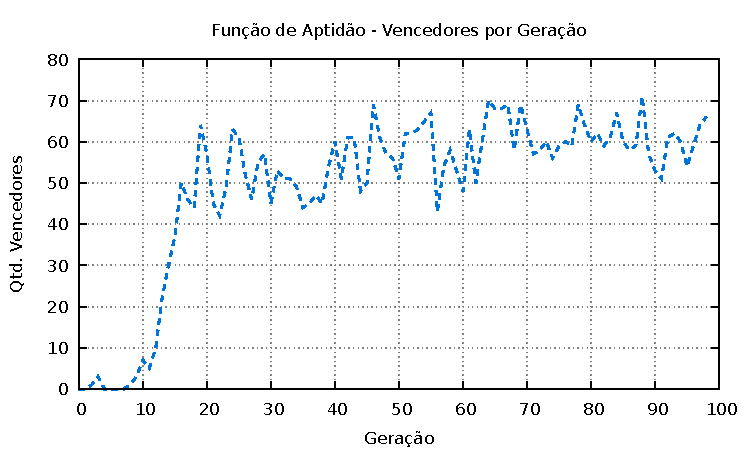
\includegraphics[width=\textwidth]{fig/extra3-winners.pdf}
        \caption{Número de organismos vencedores por geração para o cenário
        \textit{extra 3}.}
	\end{subfigure}

    \caption{Resultado da execução do cenário \textit{extra 3}.}
	\label{fig:extra3-results}
\end{figure}

Os resultados mostram que, embora o jogador tenha demorado algumas gerações até
conseguir passar do nível, ele conseguiu aprender a correr. Concluímos que a
adição da possibilidade de correr, além de permitir que os agentes passem por
áreas que necessitam de impulso para que sejam superadas, também permite que o
jogador chegue ao final do nível mais rapidamente. No caso do \textit{Spelunky},
por exemplo, isto é uma vantagem interessante, pois significa que o jogador terá
menos chances de encontrar com o inimigo \textit{fantasma} (Capítulo
\ref{chap:spelunky}, Seção \ref{sub:ghost}). Além disso, consideramos que os
melhores agentes são aqueles que chegam ao final do nível no menor tempo
possível, assim, a possibilidade de correr faz com que o agente possa chegar
antes na porta de saída.
